\subsection{Ejercicio 1}
\graphicspath{ {img/01} }


\subsubsection{Generación claves RSA Cryptool}

Para la creación de un par de claves con Cryptool 1 debemos empezar creando un perfil haciendo click en la pestaña Firmas digitales PKI, dentro del apartado PKI y luego `Generar claves'.
Dentro de este apartado deberemos seleccionar la opción RSA e indicar el número de bits para la clave, en nuestro caso 2048.
Además, deberemos de introducir un nombre de usuario al que asignaremos la clave y una clave PIN. (Figura \ref{fig:RSA-profile})

\begin{figure}[H]
    \centering
    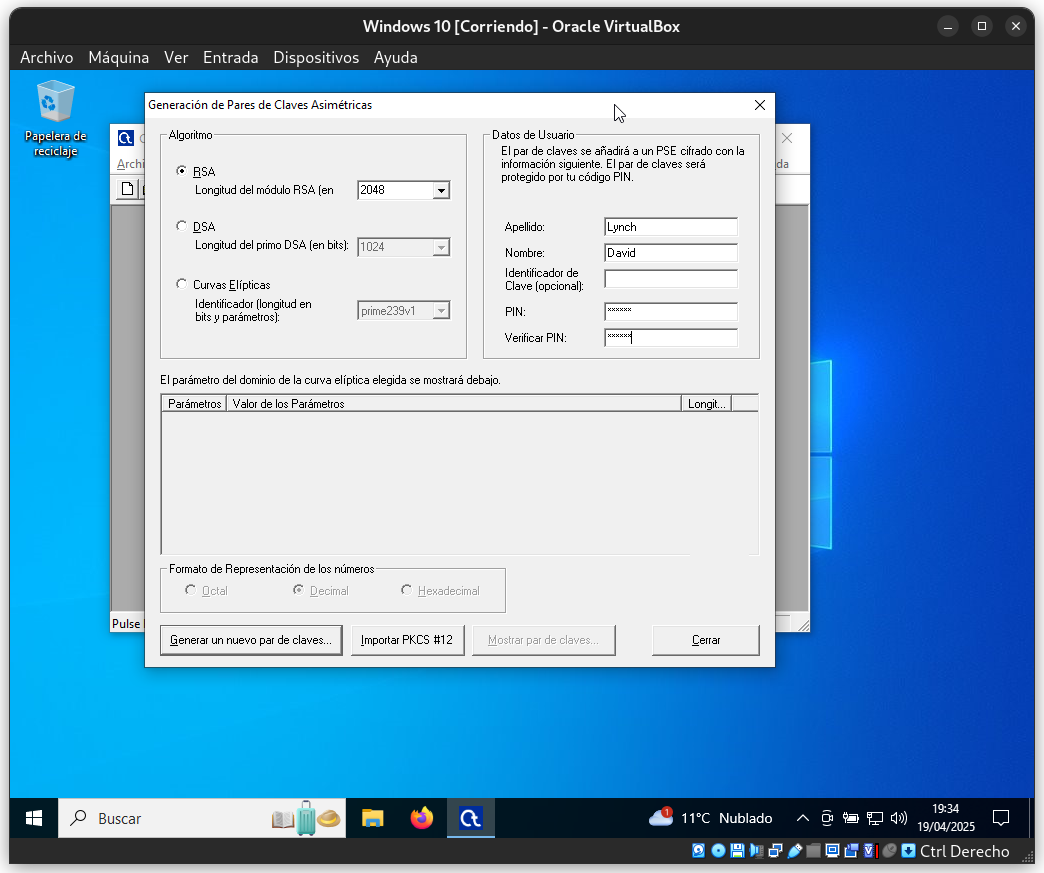
\includegraphics[width=0.8\textwidth]{ClavesRSA-01.png}
    \caption{Generación del perfil del par de claves RSA}
    \label{fig:RSA-profile}
\end{figure}

Después de esto tendremos el perfil creado y podremos acceder a sus parámetros públicos, como en la figura \ref{fig:RSA-public-params}.

\begin{figure}[H]
    \centering
    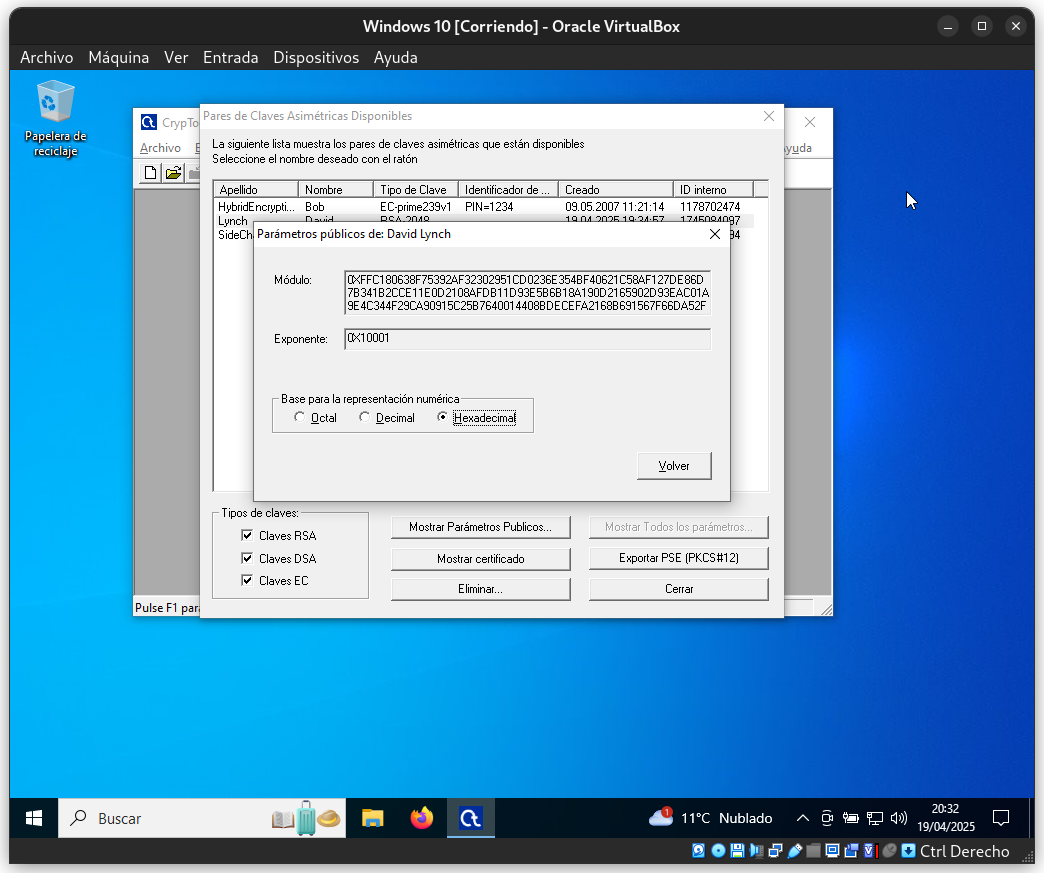
\includegraphics[width=0.8\textwidth]{ClavesRSA-02.png}
    \caption{Parámetros públicos de la clave (n, e)}
    \label{fig:RSA-public-params}
\end{figure}


\subsubsection{¿Qué números conforman la clave pública?}

La clave pública está formada principalmente por dos números. El primero de ellos es el módulo $n$, que consiste en el producto de dos números primos ($p$ y $q$ vistos en las clases teóricas) y es común tanto a la clave pública como a la privada. El segundo es el exponente público $e$, que suele tomar el valor de 65537 (el cuarto número de Fermat, F4).

\subsubsection{¿A qué nos referimos con tamaño de clave?}

Como se explica en el apartado anterior, la clave está formada por dos números: $n$ y $e$. Que la clave tenga 2048 bits significa que el módulo $n$ tiene ese tamaño.

Este tamaño nos indica la dificultad que tendría un ataque de fuerza bruta y el tamaño máximo a cifrar con esa clave. 


\subsubsection{Pruebas cifrado y descifrado}

Para el cifrado del archivo \texttt{secreto.txt} debemos abrirlo en Cryptool con la pestaña `Archivo' y accediendo a la ubicación del archivo. En nuestro caso abriremos el archivo \texttt{secreto.txt}, como se muestra en la figura \ref{fig:RSA-secreto}.

\begin{figure}[H]
    \centering
    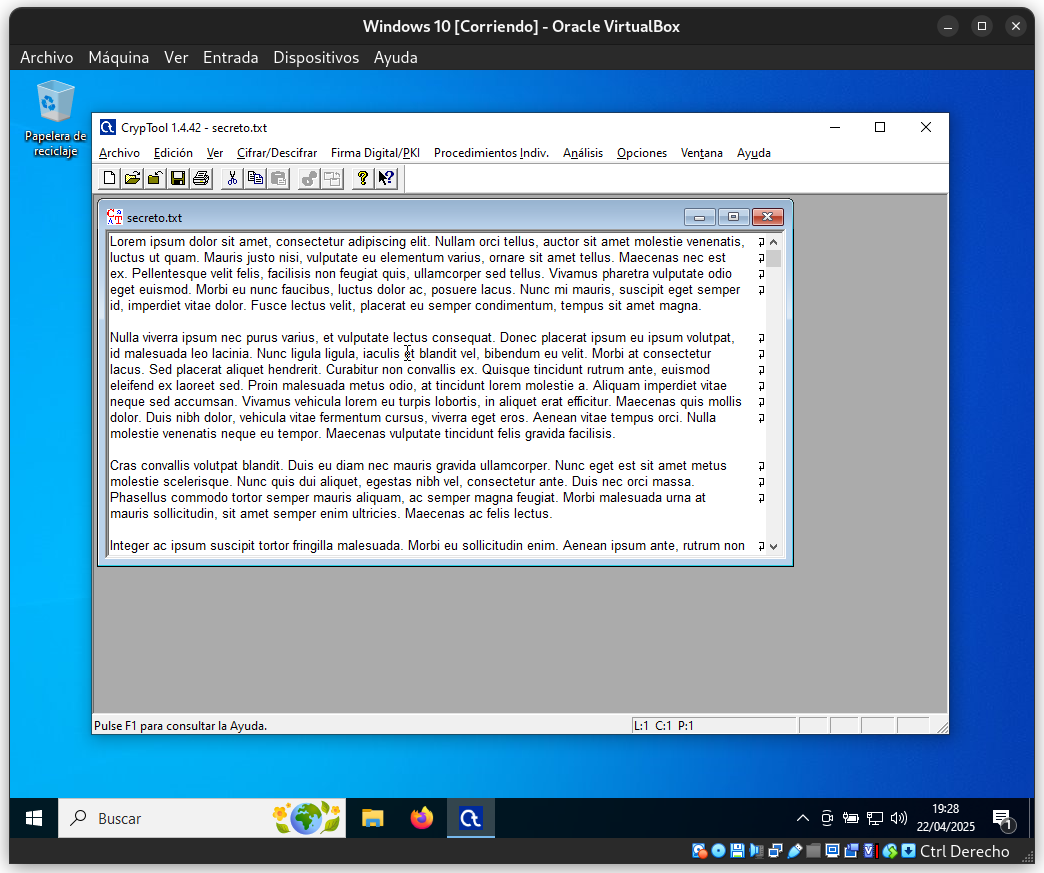
\includegraphics[width=0.8\textwidth]{EncriptadoRSA-1}
    \caption{Texto \texttt{secreto.txt} para cifrar}
    \label{fig:RSA-secreto}
\end{figure}

Posteriormente, debemos de hacer click en la pestaña `Cifrar/Descifrar', dentro de la pestaña `RSA' del apartado `Asimétrico'. Además, debemos de marcar una opción que nos saldrá en la esquina inferior izquierda para poder visualizar el tiempo de ejecución.
Como podemos observar en las figuras \ref{fig:RSA-ciph-time} y \ref{fig:RSA-deciph-time}, el tiempo de cifrado es mucho menor que el de descifrado. Si comparamos los tiempos de ejecución con un algoritmo simétrico como AES, vemos que son relativamente parecidos. Estas dos situaciones seguramente se produzcan debido a que, en RSA, utilizamos un número $e = 65537_{(10} = 10000000000000001_{(2}$, el cual permite sacar mayor partido al algoritmo de exponenciación binaria por su bajo peso de Hamming, mientras que el exponente de la clave privada no suele o no tiene por qué tener un peso de Hamming bajo.
A su vez, un algoritmo como AES utiliza el mismo procedimiento con la misma clave, por lo que los tiempos de ejecución de cifrado/descifrado tiene sentido que sean similares.

A continuación se mostrarán las salidas después de encriptar y desencriptar el archivo \texttt{secreto.txt} con nuestro par de claves creadas (figuras de la \ref{fig:RSA-ciph-time} a la \ref{fig:RSA-deciph}), respectivamente.

\begin{figure}[H]
    \centering
    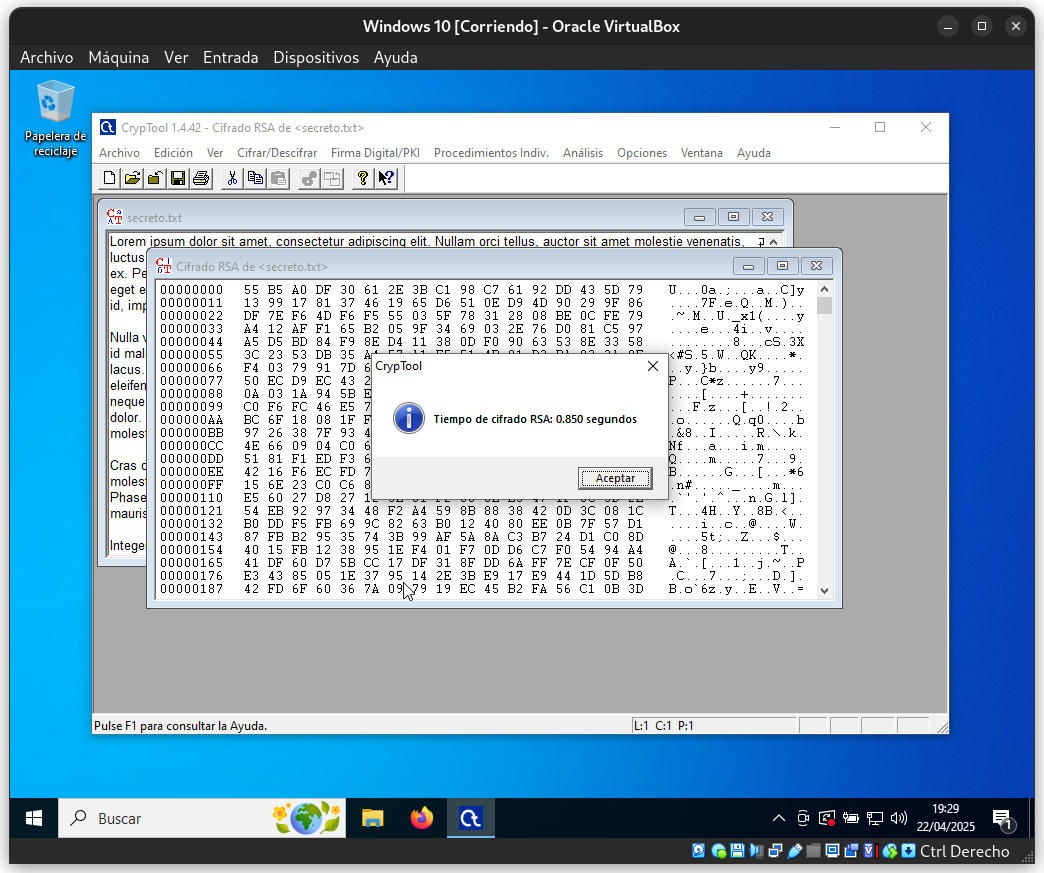
\includegraphics[width=0.8\textwidth]{EncriptadoRSA-2}
    \caption{Tiempo de ejecución del cifrado}
    \label{fig:RSA-ciph-time}
\end{figure}

\begin{figure}[H]
    \centering
    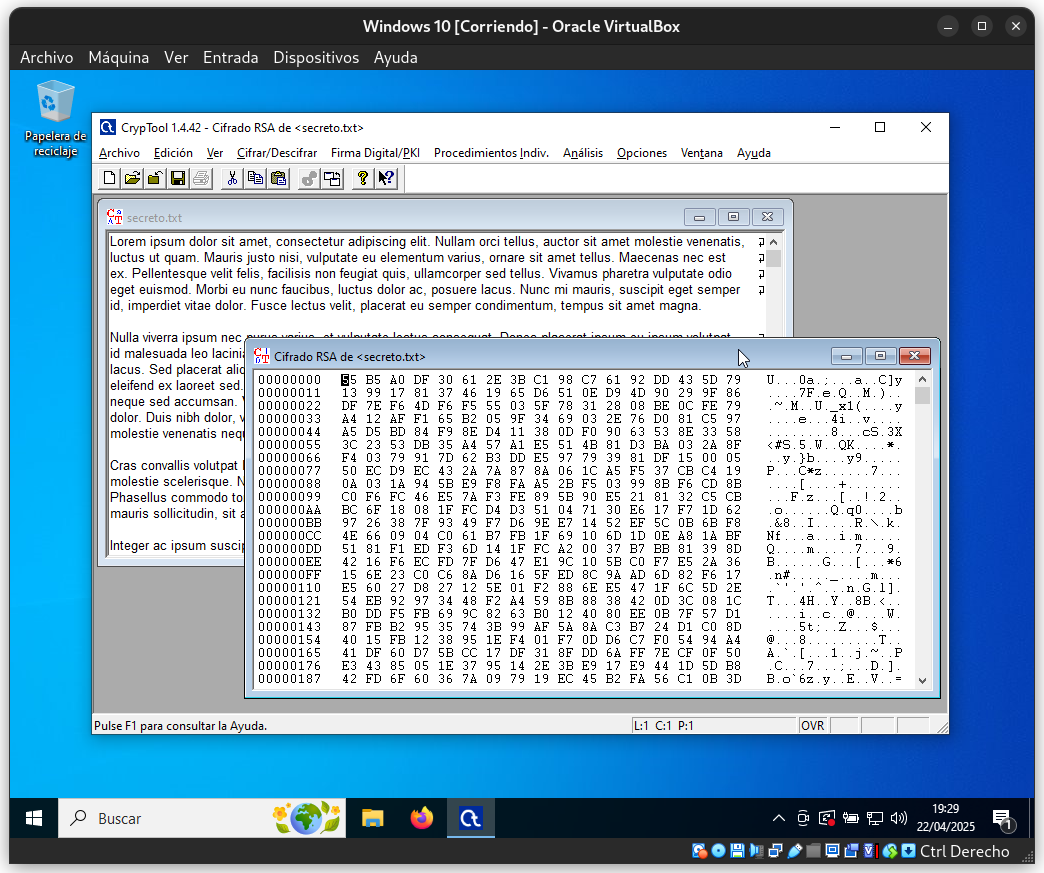
\includegraphics[width=0.8\textwidth]{EncriptadoRSA-3}
    \caption{Resultado del cifrado}
    \label{fig:RSA-ciph}
\end{figure}

\begin{figure}[H]
    \centering
    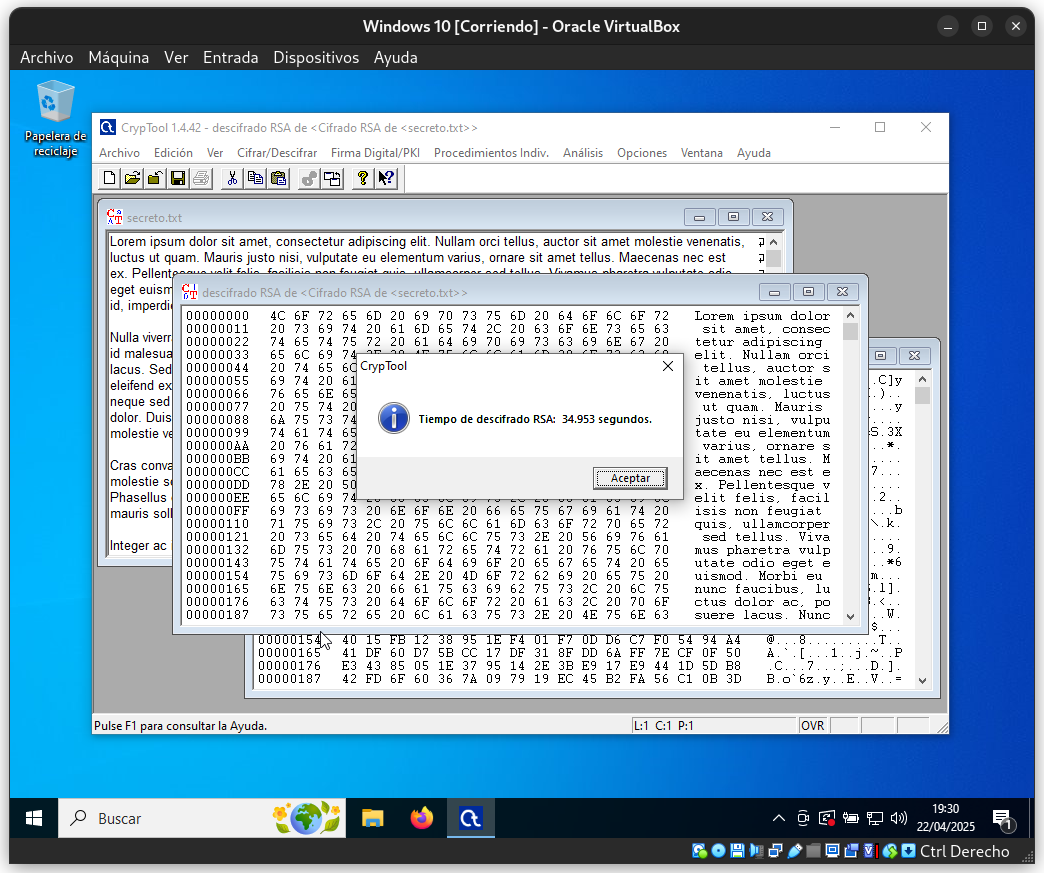
\includegraphics[width=0.8\textwidth]{DesencriptadoRSA-1}
    \caption{Tiempo de ejecución del descifrado}
    \label{fig:RSA-deciph-time}
\end{figure}

\begin{figure}[H]
    \centering
    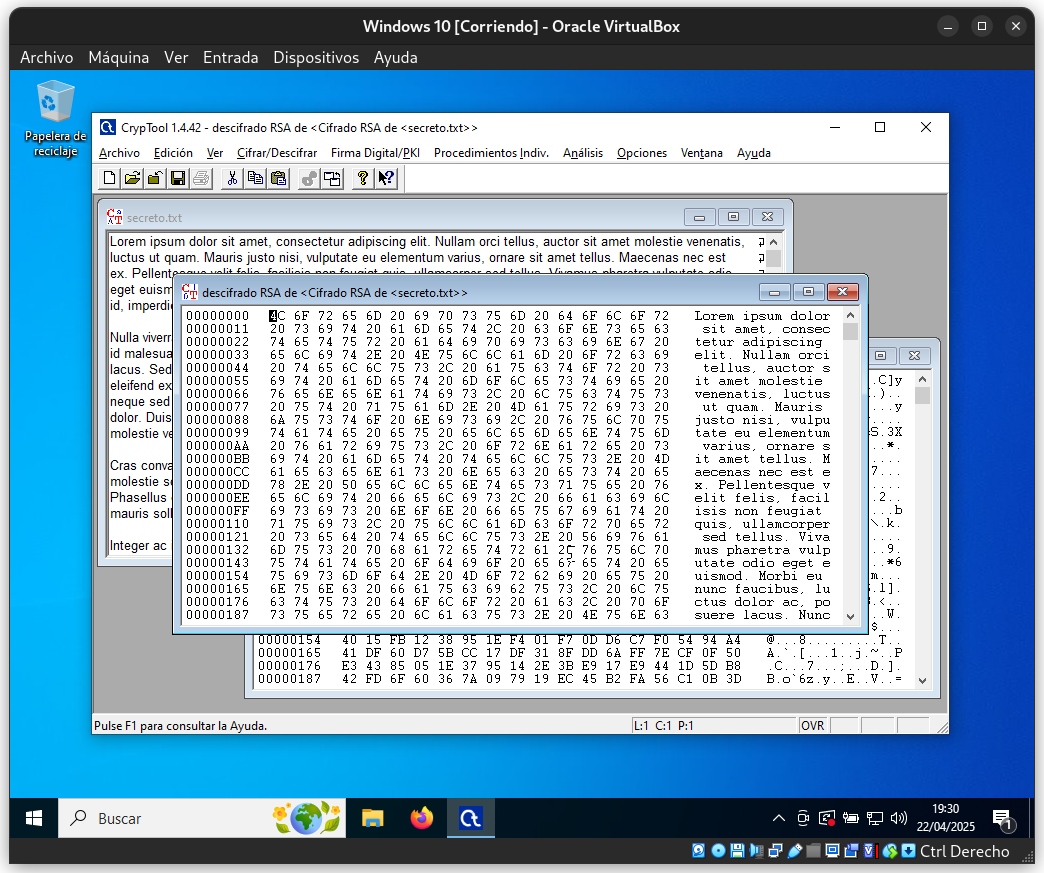
\includegraphics[width=0.8\textwidth]{DesencriptadoRSA-2}
    \caption{Resultado de descifrar el mensaje}
    \label{fig:RSA-deciph}
\end{figure}
